%%%%%%%%%%%%%%%%%%%%%%%%%%%%%%%%%%%%%%%%%
% Beamer Presentation
% LaTeX Template
% Version 1.0 (10/11/12)
%
% This template has been downloaded from:
% http://www.LaTeXTemplates.com
%
% License:
% CC BY-NC-SA 3.0 (http://creativecommons.org/licenses/by-nc-sa/3.0/)
%
%%%%%%%%%%%%%%%%%%%%%%%%%%%%%%%%%%%%%%%%%

%----------------------------------------------------------------------------------------
%	PACKAGES AND THEMES
%----------------------------------------------------------------------------------------

\documentclass{beamer}

\mode<presentation> {

% The Beamer class comes with a number of default slide themes
% which change the colors and layouts of slides. Below this is a list
% of all the themes, uncomment each in turn to see what they look like.

%\usetheme{default}
%\usetheme{AnnArbor}
%\usetheme{Antibes}
%\usetheme{Bergen}
%\usetheme{Berkeley}
%\usetheme{Berlin}
%\usetheme{Boadilla}
%\usetheme{CambridgeUS}
%\usetheme{Copenhagen}
%\usetheme{Darmstadt}
%\usetheme{Dresden}
%\usetheme{Frankfurt}
%\usetheme{Goettingen}
%\usetheme{Hannover}
%\usetheme{Ilmenau}
%\usetheme{JuanLesPins}
%\usetheme{Luebeck}
\usetheme{Madrid}
%\usetheme{Malmoe}
%\usetheme{Marburg}
%\usetheme{Montpellier}
%\usetheme{PaloAlto}
%\usetheme{Pittsburgh}
%\usetheme{Rochester}
%\usetheme{Singapore}
%\usetheme{Szeged}
%\usetheme{Warsaw}

% As well as themes, the Beamer class has a number of color themes
% for any slide theme. Uncomment each of these in turn to see how it
% changes the colors of your current slide theme.

%\usecolortheme{albatross}
%\usecolortheme{beaver}
%\usecolortheme{beetle}
%\usecolortheme{crane}
%\usecolortheme{dolphin}
%\usecolortheme{dove}
%\usecolortheme{fly}
%\usecolortheme{lily}
%\usecolortheme{orchid}
%\usecolortheme{rose}
%\usecolortheme{seagull}
%\usecolortheme{seahorse}
%\usecolortheme{whale}
%\usecolortheme{wolverine}

%\setbeamertemplate{footline} % To remove the footer line in all slides uncomment this line
%\setbeamertemplate{footline}[page number] % To replace the footer line in all slides with a simple slide count uncomment this line

%\setbeamertemplate{navigation symbols}{} % To remove the navigation symbols from the bottom of all slides uncomment this line
}

\usepackage{graphicx} % Allows including images
\usepackage{booktabs} % Allows the use of \toprule, \midrule and \bottomrule in tables

%----------------------------------------------------------------------------------------
%	TITLE PAGE
%----------------------------------------------------------------------------------------

\title[MongoDB vs OrientDB]{MongoDB vs OrientDB} % The short title appears at the bottom of every slide, the full title is only on the title page

\author{Stefano Campese} % Your name
%\institute[] % Your institution as it will appear on the bottom of every slide, may be shorthand to save space
%{
%University of California \\ % Your institution for the title page
%\medskip
%\textit{john@smith.com} % Your email address
%}
\date{\today} % Date, can be changed to a custom date

\begin{document}

\begin{frame}
\titlepage % Print the title page as the first slide
\end{frame}

\begin{frame}
\frametitle{Overview} % Table of contents slide, comment this block out to remove it
\tableofcontents % Throughout your presentation, if you choose to use \section{} and \subsection{} commands, these will automatically be printed on this slide as an overview of your presentation
\end{frame}

%----------------------------------------------------------------------------------------
%	PRESENTATION SLIDES
%----------------------------------------------------------------------------------------

%------------------------------------------------
\section{Introduction} % Sections can be created in order to organize your presentation into discrete blocks, all sections and subsections are automatically printed in the table of contents as an overview of the talk
%------------------------------------------------

%\subsection{Subsection Example} % A subsection can be created just before a set of slides with a common theme to further break down your presentation into chunks

\begin{frame}
\frametitle{MongoDB}
Born in 2009, it is one of the best known and document databases used in the world of its main features are:
\begin{itemize}
\item C++ implementation language 
\item Database model \emph{Document Store}
\item NO-SQL and Non-relational database
\item ACID transaction less
\item Ad hoc query language
\item Aggregation
\item Unique Index
\end{itemize}
\end{frame}

%------------------------------------------------

\begin{frame}
\frametitle{OrientDB}
Born in 2010, it is a hybrid between a database of documents to a database graphs. \\
Its main features are:
\begin{itemize}
\item Java implementation language
\item Database model \emph{Document Store - Graph DBMS}
\item NO-SQL Database  
\item Query language similar to SQL
\item ACID transaction
\item Multithread indexing
\item Trigger
\end{itemize}
\end{frame}

%------------------------------------------------
\section{Choose the right Database}

\begin{frame}
\frametitle{When use MongoDB}
\begin{columns}[c] % The "c" option specifies centered vertical alignment while the "t" option is used for top vertical alignment

\column{.45\textwidth} % Left column and width
\textbf{Why use MongoDB?}
\begin{enumerate}
\item Large amounts of data
\item No transactions needs
\item No relations need
\item Agile development method
\item Scalability
\item Performance
\end{enumerate}

\column{.5\textwidth} % Right column and width

\includegraphics[width=1.2\linewidth]{mongodb.png}

\end{columns}
\end{frame}


%------------------------------------------------

\begin{frame}
\frametitle{When use OrientDB}
\begin{columns}[c] % The "c" option specifies centered vertical alignment while the "t" option is used for top vertical alignment

\column{.45\textwidth} % Left column and width
\textbf{Why use OrientDB?}
\begin{enumerate}
\item Large amounts of data
\item Transactions needs
\item Telations need
\item Agile development method
\item Scalability
\item Performance (JOIN included)
\item Query language
\item Object class mapping
\end{enumerate}

\column{.5\textwidth} % Right column and width

\includegraphics[width=1\linewidth]{orientdb.png}

\end{columns}
\end{frame}

%------------------------------------------------
\section{MongoDB VS OrientDB}
%------------------------------------------------

\begin{frame}
\frametitle{MongoDB VS OrientDB}

\begin{block}{Relazioni}
\begin{itemize}
\item OrientDB: Relation whit \emph{pointer} between JSON
\item MongoDB: \emph{Index} write on file
\end{itemize}
\end{block}

\begin{block}{Query Language}
\begin{itemize}
\item OrientDB: simil-SQL language
\item MongoDB: new dedicated language 
\end{itemize}
\end{block}

\begin{block}{Memory Management}
\begin{itemize}
\item OrientDB: PLOCAL technique
\item MongoDB:  LOCAL technique
\end{itemize}
\end{block}

\begin{block}{Indexing}
\begin{itemize}
\item OrientDB: three algorithms (SB-tree, Hash index ,Lucene)
\item MongoDB:  one algorithm (B-tree)
\end{itemize}
\end{block}

\end{frame}


%------------------------------------------------
\section{Example}
%------------------------------------------------

\begin{frame}
\frametitle{Figure}
\begin{figure}
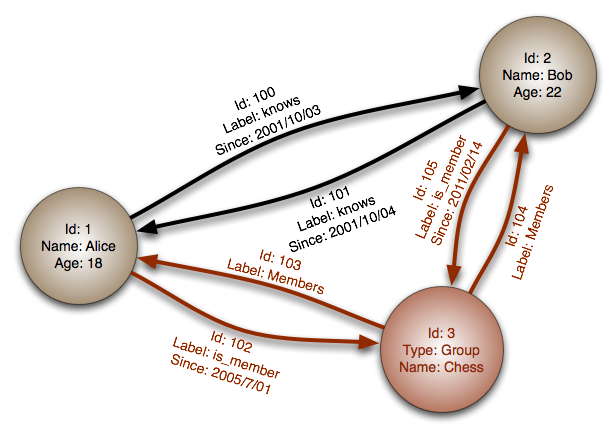
\includegraphics[width=0.8\linewidth]{GraphDatabase_PropertyGraph.png}
\caption{OrientDB vertex example}
\end{figure}
\end{frame}

%------------------------------------------------

\begin{frame}
\frametitle{Figure}
\begin{figure}
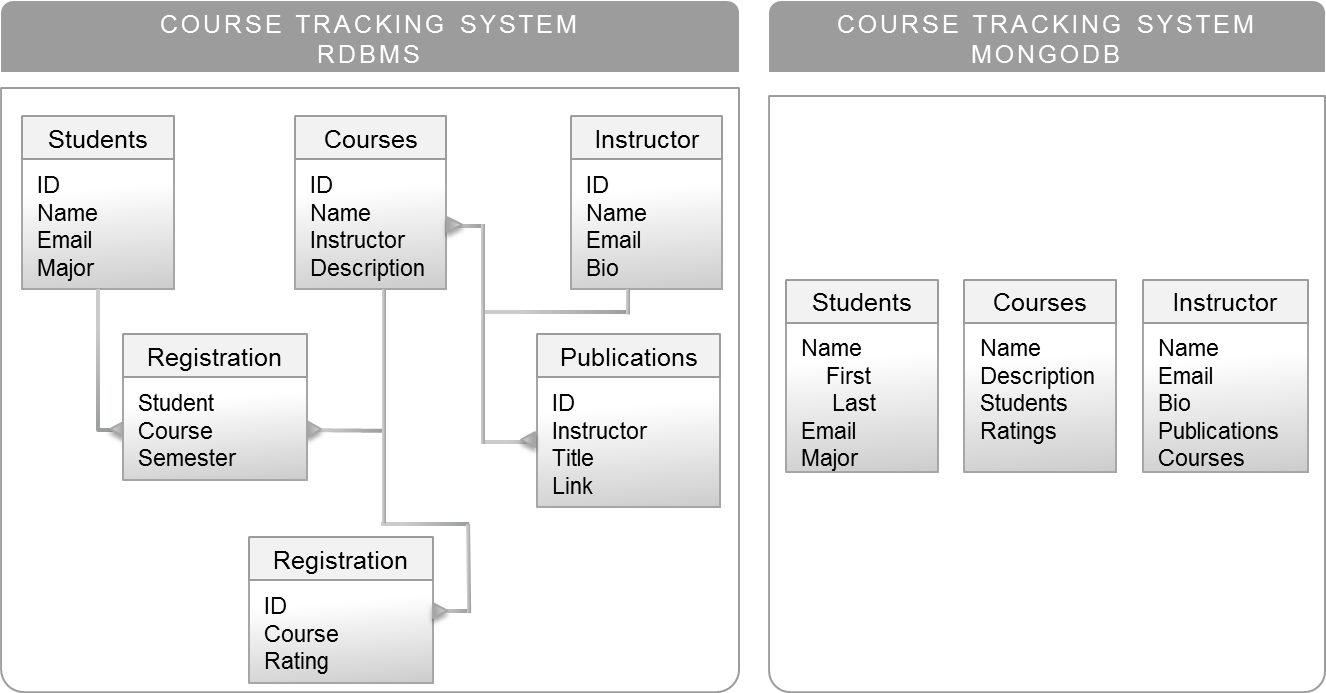
\includegraphics[width=0.8\linewidth]{01_mongodb_courses.png}
\caption{SQL to MongoDB schema}
\end{figure}
\end{frame}


%------------------------------------------------

%\begin{frame}
%\frametitle{References}
%\footnotesize{
%\begin{thebibliography}{99} % Beamer does not support BibTeX so references must be inserted manually as below
%\bibitem[Smith, 2012]{p1} John Smith (2012)
%\newblock Title of the publication
%\newblock \emph{Journal Name} 12(3), 45 -- 678.
%\end{thebibliography}
%}
%\end{frame}

%------------------------------------------------

\begin{frame}
\Huge{\centerline{End}}
\end{frame}

%----------------------------------------------------------------------------------------

\end{document}